% !TEX root = ../../Main.tex
\section{Financial Markets and Trading}

Financial markets move capital between those who have it and those who need it. In these markets, participants trade assets, hedge risk and raise funds. Each type of market has a different purpose, and \Cref{Tables:FinancialMarkets} summarises the main ones. The markets are connected. A movement in one often passes on to the others, so none of them is studied on its own. The market participants themselves set the prices. They range from private investors to banks and investment funds. Regulators set the rules that these participants must follow. Electronic platforms and algorithmic execution have opened the markets to more participants and have made prices adjust faster \cite{brandimarte_introduction_2018}.

% !TEX root = ../Main.tex
\begin{table}[htb!]
\centering
\footnotesize
\caption{Summary of Financial Markets and their Economic Role \cite{brandimarte_introduction_2018}.}
\label{Tables:FinancialMarkets}
\begin{tabularx}{\textwidth}{@{}lXl@{}}
\toprule
\textbf{Market} & \textbf{Economic Role} & \textbf{Asset Examples} \\
\midrule
Equity Market & Raising capital by trading company shares. & Stocks, Equities \\
\addlinespace
Bond Market & Debt financing, where entities borrow from investors. & Government and Corporate Bonds \\
\addlinespace
Commodities Market & Trading basic raw materials and agricultural goods. & Oil, Gold, Wheat \\
\addlinespace
Forex Market & Currency exchange for international trade. & USD, EUR, JPY, GBP \\
\addlinespace
Derivatives Market & Trading contracts for hedging or speculation. & Futures, Options, Swaps \\
\addlinespace
Indices Market & Combining and tracking the performance of a market or sector. & S\&P 500, NASDAQ \\
\addlinespace
Cryptocurrency Market & Exchanging digital currencies. & Bitcoin, Ethereum \\
\bottomrule
\end{tabularx}
\end{table}

\subsection{Forex Market: Characteristics and Significance}

The Foreign Exchange market, or Forex market, is where currencies are exchanged. It is the largest financial market by turnover. In April 2025 it traded 9.6 trillion US dollars per day on average, 28\% more than the 7.5 trillion recorded three years earlier. It trades continuously across time zones, because the banks and institutions that quote its prices are spread around the world. Spot transactions, the instrument traded in this work, make up 3 trillion of that daily total. The US Dollar is on one side of 89.2\% of all trades, and the ten most traded currency pairs all include it \cite{bis_otc_2025}. Prices react to interest rate decisions, economic releases and political events. Participants normally trade with leverage. Leverage allows a position much larger than the capital deposited, and it scales profits and losses in the same proportion. Its market depth, its continuous operation, its sensitivity to news and the routine use of leverage make it suitable for automated trading. The same properties make it hard to model. Its behaviour is noisy and non-stationary, which means that its statistical properties change over time. This is why adaptive, data-driven strategies are of interest \cite{donnelly_art_2019}.

\subsection{Forex Trading: Fundamental Concepts and Operation}

Trading a currency pair means buying one currency and selling another at the same time. Buying the EUR/USD pair means buying Euros and selling US Dollars, expecting that the Euro will strengthen against the US Dollar. This work uses the seven major currency pairs: EUR/USD, USD/JPY, GBP/USD, AUD/USD, USD/CHF, NZD/USD and USD/CAD. They are built from the Euro (EUR), US Dollar (USD), Japanese Yen (JPY), British Pound (GBP), Australian Dollar (AUD), Swiss Franc (CHF) and New Zealand Dollar (NZD). Every one of them has the US Dollar on one side. Deciding whether to buy or sell a pair comes down to predicting the strength of one currency relative to the other \cite{donnelly_art_2019}.

A position is the exposure a trader holds in a pair. It is the amount of the pair that the trader has bought or sold and not yet closed. A long position makes money when the pair rises and loses money when it falls. A short position does the opposite. A currency pair is a ratio between two currencies, so short selling is as natural as buying and needs no borrowing. In equity markets this is not the case. Positions are opened and closed with orders. A market order is executed at once, at the price quoted at that moment. A limit order is executed only at a given price or better. A stop order is executed once the price passes a given level. Two stop orders are often attached to an open position. A stop loss closes the position when the loss reaches a chosen level. A take profit closes it when a target is reached.

Forex trading takes place in a decentralised market that works worldwide. There is no single exchange where all trades happen. Instead, trades are handled by a network of market makers and brokers. The market makers are mainly banks, and the market between them is known as the interbank market. Interbank trades are large, and most of them are made by institutions such as multinational companies and large hedge funds. Retail traders take part through brokers, who have access to that network and act as intermediaries. Market makers and brokers always quote two prices. The bid price is the price at which they will buy the pair. The ask price is the price at which they will sell it. The difference between the two is the spread. Without a central trading venue, one might expect the market to be poorly regulated. However, competition between market makers keeps their quoted prices close to one another and keeps spreads narrow \cite{donnelly_art_2019}.

Traders look at prices on charts, and the candlestick chart is the standard type. A candlestick chart is made of candlesticks. Each one shows how the price moved over a period of time, which can be anything from minutes to years. A tick is a single update of the quoted price. It is published whenever a market maker changes its bid or its ask. The name comes from its shape, which looks like a candle with a wick at both ends. Each candlestick shows the opening price (O), the highest price (H), the lowest price (L) and the closing price (C) of its period (see \Cref{Figure:CandlestickChart}). The colour of the candlestick shows the direction of the move. A lighter shade means the price went up, and a darker shade means it went down. This lets traders see the direction of the market quickly, just by looking at the chart. Candlestick charts do not show volume (V), which is normally drawn separately below the price. Forex has no central venue, so there is no consolidated record of traded size. Brokers report tick volume instead, which is the number of quote updates in the period. This work uses tick volume throughout \cite{rhoads_candlestick_2022}.

\begin{figure}[htb!]
\centering
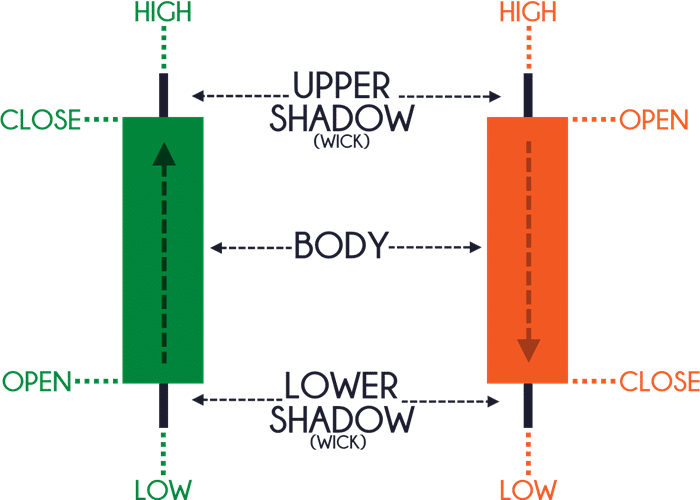
\includegraphics[width=0.4\textwidth]{Images/CandlestickChart.png}
\caption{Candlesticks showing upward (bullish) and downward (bearish) movements respectively \cite{teo_candlestick_nodate}.}
\label{Figure:CandlestickChart}
\end{figure}

This work uses tick data as its main record, because it has the finest resolution the broker provides. Whenever a coarser view is needed, it computes from the ticks the opening, highest, lowest and closing prices and the tick volume, called OHLCV data for short \cite{rhoads_candlestick_2022}. Indicators computed from that data give the model more context, as described below.

\subsection{Forex Costs: Spreads, Commissions and Overnight Financing}

Trading is not free, and its costs are large compared with the profit a single position can make. Three costs apply in Forex, and each is charged separately from the others. Prices are quoted in units that depend on the pair. A pip is the fourth decimal place of the quote for most pairs, or the second for pairs quoted against the Japanese Yen. A point is one tenth of a pip. It is the smallest price increment a broker quotes. The size of a position is given in units of the base currency, the first currency of the pair, and one standard lot is $100{,}000$ units. For a position of volume $q$ at price $p$, the notional value, which is the value of the position in the quote currency (the second currency of the pair), is

\begin{equation}
V = q \cdot p
\end{equation}

The \textbf{spread} is the first cost. It is an implicit cost, paid through the price. A position is opened at the ask and closed at the bid, so a full round trip, opening and then closing, crosses the spread once. For a position of volume $q$, the cost is

\begin{equation}
C_{spread} = (p_{ask} - p_{bid}) \cdot q
\label{Equation:SpreadCost}
\end{equation}

The spread is not constant. It widens when liquidity falls, around economic releases and at the daily rollover. A strategy tested with a fixed spread is therefore tested on a market that does not exist in practice.

The \textbf{commission} is the second cost, and it is an explicit cost. Some accounts quote the raw interbank spread. On these accounts the broker makes its money through a commission charged on the traded volume, instead of through a wider spread. If the commission is given as a number of points $c$, and $s_{point}$ is the size of one point, the cost of a position of volume $q$ is

\begin{equation}
C_{commission} = c \cdot s_{point} \cdot q
\label{Equation:CommissionCost}
\end{equation}

The spread and the commission are separate costs, and a trader pays both. On a raw-spread account, treating the spread as if it already included the commission makes trading look cheaper than it is.

The \textbf{swap}, or overnight financing, is the third cost. It comes from the interest rate differential between the two currencies of the pair. It is charged when a position is still open at the daily rollover, the moment when the trading day ends. On one day of the week the charge is multiplied, to cover the weekend. Depending on the direction of the position and the sign of the differential, the swap can be a cost or a credit. Some account types remove it completely, so that clients can avoid interest for religious reasons. These are known as swap-free accounts. Finally, leverage decides how much capital a position needs. With leverage $L$, the margin, which is the capital set aside for a position of notional value $V$, is

\begin{equation}
M = \frac{V}{L}
\end{equation}

Leverage does not change the profit or loss of a position. It only changes the capital set aside for it. So leverage affects the return of the account, and the return of the trade stays the same. These costs are not the same on every type of account. Choosing the account is therefore part of designing a strategy. A raw-spread account quotes the interbank spread with no markup and makes its money through the commission. This makes the total cost of a position lower. It also makes the cost explicit, which is more useful. The implicit part of the cost is reduced to the market spread, and the rest is a published rate. A swap-free account charges no overnight financing at all. An account with both features suits a strategy that holds positions for days. Such a strategy pays the spread and the commission only a few times per position, but it would otherwise pay financing for every night the position stays open. This work is evaluated on an account that has both features. The spread and the commission are therefore the only costs applied, and the financing cost is exactly zero, so it does not need to be estimated.

\subsection{Financial Analysis: Main Types and Formulas}

Representing the data is one half of the problem. The other half is analysing it to decide what to trade. Financial analysis is usually divided into three types \cite{lim_handbook_2015}:

\begin{itemize}
\item \textbf{Fundamental Analysis}: studies the economic factors that affect currency prices. These include GDP growth, employment rates, interest rates and monetary policy, which help to predict currency trends from the economic health of a country. However, much of this data is qualitative. This makes it hard to use in computer models, which work best with structured numerical input.
\item \textbf{Sentiment Analysis}: tries to measure the mood of the market by analysing news, market commentary and similar qualitative data. It aims to measure how the shared emotions of traders affect market trends. It is complex and needs advanced natural language processing, so it is harder to include in a model.
\item \textbf{Technical Analysis}: analyses past OHLCV data to predict future market movements. It assumes that past market behaviour will repeat itself, so patterns or measures found in current data can predict future movements. It is preferred because its results are numbers, which complex machine learning models can use.
\end{itemize}

Of the three, this work uses technical analysis. It produces numerical series directly from price data, so a model can use them without any further interpretation. Technical analysis is divided into indicators and candlestick patterns. Indicators are measures calculated from past market data, created mainly by mathematicians and economists. They give a numerical view of how the market moves. They are usually grouped into four main types \cite{lim_handbook_2015}:

\begin{itemize}
\item \textbf{Trend Indicators}: Used to find the main direction of the market by filtering out market noise. See \Cref{Tables:TrendIndicators} for details of frequently used indicators.
\item \textbf{Momentum Indicators}: Used to measure the momentum of a trend, whether it is strong or weak, and whether a reversal is expected. See \Cref{Tables:MomentumIndicators} for details of frequently used indicators.
\item \textbf{Volume Indicators}: Used to look at the trading volume, which gives clues about the strength of a price movement. See \Cref{Tables:VolumeIndicators} for details of frequently used indicators.
\item \textbf{Volatility Indicators}: Used to measure the level of uncertainty or risk that comes with the volatility of the price. See \Cref{Tables:VolatilityIndicators} for details of frequently used indicators.
\end{itemize}


The four tables list indicators in common use. They do not describe the contents of any one system. The framework built for this work implements the moving average family and the crossovers between its members, the Rate of Change, the Moving Average Convergence Divergence, the Average True Range, the Realised Volatility and the Efficiency Ratio. It implements no volume indicators. The tick volume a Forex broker reports counts quote updates, not traded size, and this limits what those indicators can measure. Ten instances of the implemented set form the observation the agent receives. They are listed in \Cref{Chapter:Implementation}. Candlestick patterns work differently. They do not compute a value. They describe shapes, formed by one or more candlesticks, that traders link to a change in behaviour \cite{rhoads_candlestick_2022}. Such patterns can be encoded as numbers and given to a model in the same way as an indicator \cite{jansen_machine_2020}. This work does not use them. The observation is built from indicators only.

\subsection{Performance Measurement: Returns, Risk and Ratios}
\label{Section:PerformanceMeasurement}

A trading strategy is judged by what it earns and by the risk it takes to earn it. A single return figure is therefore not enough to compare two strategies. The measures below are the ones reported in \Cref{Chapter:ExperimentalResults}. They are defined on an equity series, which is the value of the account over time. They therefore apply without change to a portfolio of several strategies. They are then computed on the combined equity of the portfolio, and not on each strategy separately. This matters because the risk of a portfolio depends on how its parts move together, and not only on the risk of each part.

The total return over a period compares the final and the initial equity $E$ of the account:

\begin{equation}
R = \frac{E_{final} - E_{initial}}{E_{initial}}
\end{equation}

Periods differ in length, so returns are annualised, that is, converted to a yearly rate, before they are compared. With a duration $\Delta t$ in seconds and a year of $365$ days,

\begin{equation}
R_{annual} = (1 + R)^{\frac{365 \cdot 86400}{\Delta t}} - 1
\label{Equation:AnnualizedReturn}
\end{equation}

Risk is measured in two ways. The first is volatility, which is the standard deviation of returns, annualised by the rate at which the strategy trades. The second is drawdown. At any moment, the drawdown is the distance between the current equity and the highest equity reached so far:

\begin{equation}
D(t) = \frac{E(t) - \max_{s \leq t} E(s)}{\max_{s \leq t} E(s)}
\label{Equation:Drawdown}
\end{equation}

The maximum drawdown is the worst value of $D(t)$ over the period. It is the largest loss from a peak that an investor would have suffered. The mean drawdown is the average of $D(t)$. It shows how far below its peak the account is on a typical day, instead of at its worst moment. Four ratios combine return and risk. All of them divide an annualised excess return, which is the return above the risk-free rate, by a measure of risk. They differ only in the measure of risk they use. The absolute value of that measure is used, because a drawdown is negative under the definition above. With $R_f$ as the risk-free rate,

\begin{equation}
\text{Ratio} = \frac{R_{annual} - R_f}{\left| \text{risk} \right|}
\label{Equation:RiskRatio}
\end{equation}

The \textbf{Sharpe ratio} \cite{sharpe_sharpe_1994} uses the annualised volatility, so it penalises upward and downward moves equally. The \textbf{Sortino ratio} \cite{sortino_performance_1994} uses the downside volatility instead, computed from negative returns only. The argument is that an investor does not mind upside variability. The \textbf{Calmar ratio} uses the maximum drawdown, so it measures return against the worst loss suffered. The \textbf{Sterling ratio} uses the mean drawdown. This makes it less sensitive to a single bad period, and closer to what holding the strategy is like on a typical day. The Calmar and Sterling ratios both have several definitions in the literature, and the ones used here follow \cite{bacon_practical_2023}. By construction, the mean drawdown is smaller than the maximum drawdown. So, for a strategy with a positive excess return, the Sterling ratio is the larger of the two ratios. When the excess return is negative, the order is reversed.

\subsection{Algorithmic and Quantitative Trading}

More and more of the trading in financial markets is done by algorithms. Algorithmic trading uses computer programs to execute trades faster and in larger volume than a human can. The programs analyse large datasets, read market conditions and act on set rules. Algorithmic trading is used for pre-trade analysis, signal generation and trade execution. It is what allows institutions to run complex strategies at a large scale. Quantitative trading is a subfield of algorithmic trading. It uses mathematical and statistical models to find opportunities in market data, through the analysis of past data and through machine learning. It follows systematic rules instead of the discretionary judgement of a trader, and it needs knowledge of both finance and mathematics \cite{chan_quantitative_2021}. Together, the two have changed how markets work. They brought practices such as high-frequency trading, and they shortened the time that prices take to react to new information. They have also made machine learning central to the field. Neural networks are used to find structure in market data, and reinforcement learning is used to decide what to do with it \cite{jansen_machine_2020}. These two fields are the subject of the next sections.